\chapter{Progress}
\setcounter{secnumdepth}{4}
\setcounter{tocdepth}{4}
This document is intended to be both an example of the TU Delft \LaTeX{} template for reports and theses, as well as a short introduction to its use. It is not intended to be a general introduction to \LaTeX{} itself

Instructions on how to use this template under Windows and Linux, and which \LaTeX{} packages are required, can be found in \texttt{README.txt}.

\section{Movement between buildings}
\subsection{Bar chart}
\subsection{Maps}
In order to get an overview about how people move on the campus and further more,  find out movement patterns, a map visualization is essential. Map visualization consists of three parts: 
\begin{enumerate}
\item base map: open street map is used as base map. There are many labels on open street map, providing more context of the environment, so it is more clear and readable compared to other base maps like satellite images.
\item building markers: building markers show the locations of the buildings. Google maps marker style is used since it is commonly used in many map application. Because the shape of the building is not useful in analyzing movement patterns between buildings, each building is regarded as a point instead of a polygon, thus a node in the network, 
\item lines: lines are the most essential part in map visualization, they represent movements between buildings.
\end{enumerate}

In the first stage of map visualization, only base map and lines are taken into consideration, building markers are not shown on the map. The line width represents the amount of movement and movements are aggregated daily regardless of the timestamp of each movement during a day. This map visualization gives an overview of the movements over a day and between which buildings there are the most movements. The following maps show the difference of the amount of movement between April 11th (weekday) and April 17th (weekend).
\graphicspath{ {pics/} }
\begin{figure}[H]
\minipage{0.2\textwidth}
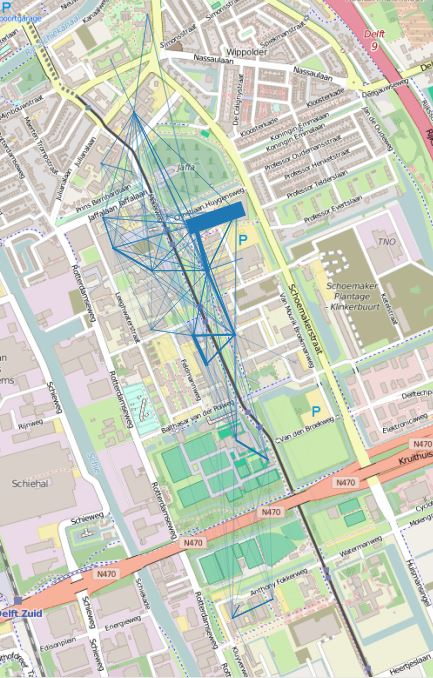
\includegraphics[scale=0.7,left]{pic1}
\captionsetup{justification=centering}
\caption{Movements of April 11th (week day)}
\endminipage\hfill
\minipage{0.2\textwidth}
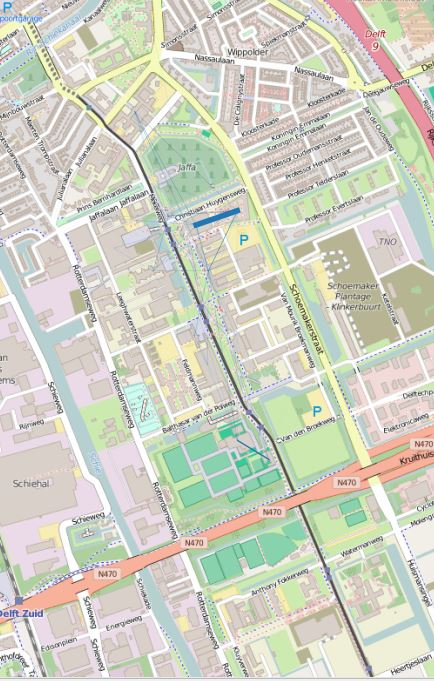
\includegraphics[scale=0.7,right]{pic2}
\captionsetup{justification=centering}
\caption{Movements of April 17th (weekend)}
\endminipage\hfill

\end{figure}
It's clear that between Aula and library, there are the most movements and the amount of movements is totally different on weekday and on weekend.

Regarding the movements are dynamic and time is also highly related to movements, a dynamic map visualization is created to display individual movement over a day with temporal information. The following screenshots of the gif file show how the movements look like at a certain time of a day:

\begin{figure}[H]
\minipage{0.2\textwidth}
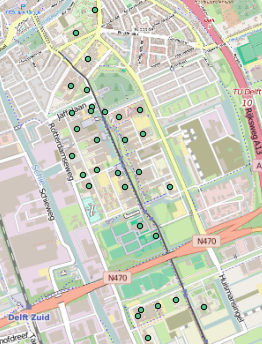
\includegraphics[scale=0.6,left]{frame009}
\captionsetup{justification=centering}
\caption{Movements of April 11th, 7:00 am}
\endminipage\hfill
\minipage{0.2\textwidth}
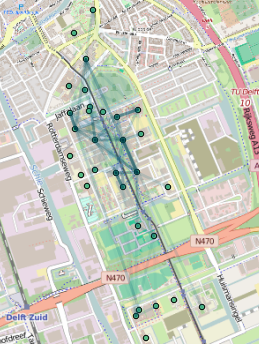
\includegraphics[scale=0.6,center]{frame021}
\captionsetup{justification=centering}
\caption{Movements of April 11th, 9:00 am}
\endminipage\hfill
\minipage{0.2\textwidth}
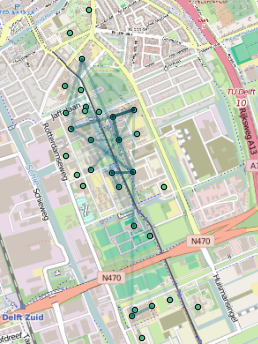
\includegraphics[scale=0.6,right]{frame033}
\captionsetup{justification=centering}
\caption{Movements of April 11th 11:00 am}
\endminipage\hfill
\end{figure}

\begin{figure}[H]
\minipage{0.2\textwidth}
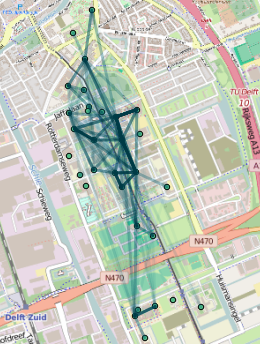
\includegraphics[scale=0.6,left]{frame045}
\captionsetup{justification=centering}
\caption{Movements of April 11th, 13:00 pm}
\endminipage\hfill
\minipage{0.2\textwidth}
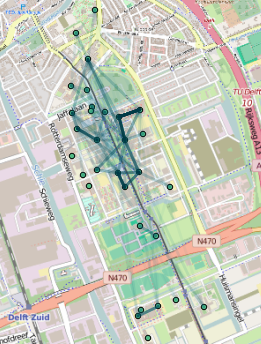
\includegraphics[scale=0.6,center]{frame057}
\captionsetup{justification=centering}
\caption{Movements of April 11th, 15:00 pm}
\endminipage\hfill
\minipage{0.2\textwidth}
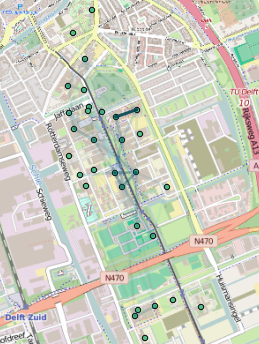
\includegraphics[scale=0.6,right]{frame066}
\captionsetup{justification=centering}
\caption{Movements of April 11th 16:30 pm}
\endminipage\hfill
\end{figure}

\begin{figure}[H]
\minipage[height=2]{0.2\textwidth}
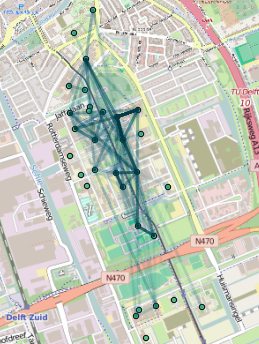
\includegraphics[scale=0.6,left]{frame075}
\captionsetup{justification=centering}
\caption{Movements of April 11th, 18:00 pm}
\endminipage\hfill
\minipage[height=2]{0.2\textwidth}
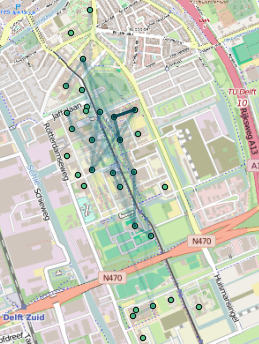
\includegraphics[scale=0.6,center]{frame087}
\captionsetup{justification=centering}
\caption{Movements of April 11th, 20:00 pm}
\endminipage\hfill
\minipage[height=2]{0.2\textwidth}
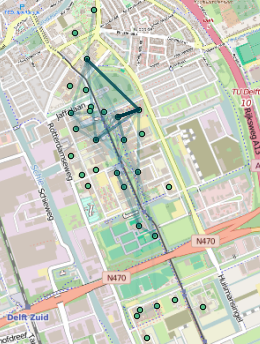
\includegraphics[scale=0.6,right]{frame099}
\captionsetup{justification=centering}
\caption{Movements of April 11th 22:00 pm}
\endminipage\hfill
\end{figure}

In these pictures, the more movements there are, the less transparent the lines are. So generally speaking, from 7:00 am to 20:00 pm, there are two peaks at 13:00 pm and 18:00 pm. Hence, it is possible to get some insights about movement patterns from the animation. However, the dynamic map visualization doesn't provide detailed information to dig into but only an overview. So in order to mine on movement patterns, it is necessary to create maps containing more information, including time, direction and so forth. 

Because the amount of data is big, it is more convenient to generate maps automatically so that it will fasten the progress of finding movement patterns. According to the three components of map, there is some information needed to be collected before visualizing movement on map. The locations of buildings are collected manually on Google earth based the campus map. These locations are exported as KML file and imported into QGIS. After adding geometry columns x and y, the csv file is created and imported into database. By using $ST\_MakePoint$ function, a geometry column is created in database. In summary, the building locations are stored as the structure described in following table:

\begin{table}[H]
\centering
\begin{tabular}{|c|c|c|c|c|}
\hline 
id & name & geometry & x & y \\
\hline
0 & world & & & \\
\hline
3 & science\_ center & 010100000042A7.. & 4.36939919846287 & 52.0072322181367 \\
\hline
5 & tnw\_ bio & 010100000043AE.. & 4.37120211221402 & 52.0086132164098 \\
\hline
8 & bk\_ city & 010100000077E3.. & 4.37053698152436 & 52.0056562098059 \\
\hline
12 & tnw\_ dct & 01010000007CA.. & 4.36891378927259 & 52.0040834950037\\
\hline
.. & ... & ....& .... &....\\
\hline	
\end{tabular}
\captionsetup{justification=centering}
\caption{Building data structure}
\label{table:1}
\end{table}

There is a special 'building' called $world$ in the database. It is not an actual location, it is a virtual location which is used if someone is not scanned on the campus in a period of time. After storing the locations of buildings in the database, these locations will be extracted automatically from database to generate maps. There are two properties of lines used to deliver information:
\begin{enumerate}
\item width: line width is used to represent the amount of movements, but the amount is aggregated for both directions.
\item color: color is gradient from red to green. Red line means the movement is not symmetric that much more people move in one direction than the other, while green line means the movement is symmetric.
\end{enumerate}

\section{Sequences}

This template will automatically generate a cover page if you issue the \texttt{\textbackslash makecover} command. There are two formats for the cover page: one with a page-filling (`bleeding')
illustration, with the title(s) and author(s) in large ultrathin typeface, and the other where the illustration fills the lower half of the A4, whereas title(s), author(s) and additional
text are set in the standard sans-serif font on a plain background with a color chosen by the user. The last option is selected by the optional key \texttt{split}: \texttt{\textbackslash makecover[split]} yields
a page with the illustration on the lower half. All illustrations are bleeding, in accordance with the TU Delft style.

Before generating the cover, you need to provide the information to put on it. This can be done with the following commands:
\begin{itemize}
\item\texttt{\textbackslash title[Optional Color]\{Title\}} \\
    This command is used to provide the title of the document. The title
    title is also printed on the spine. If you use a title page (see below), this information will be used there as well.
    As the title, subtitle and author name are printed directly over the cover photo, it will often be necessary to adjust the print color in order to have
    sufficient contrast between the text and the background. The optional color argument is used for this.
\item\texttt{\textbackslash title[Optional Color]\{Subtitle\}} \\
    This command is used to provide a subtitle for the document. If you use a title page (see below), this information will be used there as well.
    It possible to adjust the print color in order to have
    sufficient contrast between the text and the background -- the optional color argument is used for this.
\item\texttt{\textbackslash author\{J.\ Random Author\}} \\
    This command specifies the author. The default color is \texttt{tudelft-white}, but this may be adjusted in the same way as the titles.
\item\texttt{\textbackslash affiliation\{Technische Universiteit Delft\}} \\
    The affiliation is the text printed vertically on the front cover. It can be the affiliation, such as the university or department name, or be used for the document type (\emph{e.g.}, Master's thesis). The default color is again \texttt{tudelft-white}, adjustable through the \texttt{color} option.
\item\texttt{\textbackslash coverimage\{cover.jpg\}} \\
    With this command you can specify the filename of the cover image. The image is stretched to fill the full width of the front cover (including the spine if a back cover is present).
\item\texttt{\textbackslash covertext\{Cover Text\}} \\
    If a back cover is present, the cover text is printed on the back. Internally, this text box is created using the \LaTeX{} \texttt{minipage} environment, so it supports line breaks.
\item\texttt{\textbackslash titleoffsetx\{OffsetX\},\textbackslash titleoffsety\{OffsetY\}}
    If the cover page contains a page-filling picture (i.e., \texttt{split} is not specified with the \texttt{makecover} command, the best position of the title depends a lot on the picture chosen for it. The lower left corner of the minipage containing title, subtitle and author is 
    specified by these two commands. The offsets are measured from the top left corner of the page. 
\item\texttt{\textbackslash afiloffsetx\{AfilX\}, \textbackslash afiloffsety\{AfilY\}}
    specifies the lower left corner of the text containing the affiliation, measured from the top left corner of the page. 
\end{itemize}

In addition to \texttt{[split]}, the \texttt{\textbackslash makecover} command accepts several additional options for customizing the layout of the cover. 
The most important of these is \texttt{back}. Supplying this option will generate a back cover as well as a front, including the spine. Since this requires a page size slightly larger than twice A4 (to make room for the spine), and \LaTeX{} does not support different page sizes within the same document, it is wise to create a separate file for the cover. \texttt{cover.tex} contains an example. The recommended page size for the full cover can be set with
\begin{quote}
    \textbackslash geometry\{papersize=\{1226bp,851bp\}\}
\end{quote}
after the document class and before \texttt{\textbackslash begin\{document\}}.

The other options \texttt{\textbackslash makecover} accepts are
\begin{itemize}
\item\texttt{nospine} \\
    If a back cover is generated, the title will also be printed in a black box on the spine. However, for smaller documents the spine might not be wide enough. Specifying this option disables printing the title on the spine.
\item\texttt{frontbottom} \\
    By default the black box on the front is situated above the blue box. Specifying this option will place the black box below the blue one.
\item\texttt{spinewidth} \\
    If a back cover is present, this option can be used to set the width of the spine. The default is \texttt{spinewidth=1cm}.
\item\texttt{frontboxwidth}, \texttt{frontboxheight}, \texttt{backboxwidth}, \texttt{backboxheight} \\
    As their names suggest, these options are used to set the width and height of the front (black) and back (blue) boxes. The default widths and heights are \texttt{4.375in} and \texttt{2.1875in}, respectively.
\item\texttt{x}, \texttt{y} \\
    The blue and black boxes touch each other in a corner. The location of this corner can be set with these options. It is defined with respect to the top left corner of the front cover. The default values are \texttt{x=0.8125in} and \texttt{y=3in}.
\item\texttt{margin} \\
    This option sets the margin between the borders of the boxes and their text. The default value is \texttt{12pt}.
\end{itemize}

For a thesis it is desirable to have a title page within the document, containing information like the thesis committee members. To give you greater flexibility over the layout of this page, it is not generated by a command like \texttt{\textbackslash makecover}, but instead described in the file \texttt{title.tex}. Modify this file according to your needs. The example text is in English, but Dutch translations are provided in the comments. Note that for a thesis, the title page is subject to requirements which differ by faculty. Make sure to check these requirements before printing.

\section{Pre-Processing}

Each chapter has its own file. For example, the \LaTeX{} source of this chapter can be found in \texttt{chapter-1.tex}. A chapter starts with the command
\begin{quote}
    \texttt{\textbackslash chapter\{Chapter title\}}
\end{quote}
This starts a new page, prints the chapter number and title and adds a link in the table of contents. If the title is very long, it may be desirable to use a shorter version in the page headers and the table of contents. This can be achieved by specifying the short title in brackets:
\begin{quote}
    \texttt{\textbackslash chapter[Short title]\{Very long title with many words which could not possibly fit on one line\}}
\end{quote}
Unnumbered chapters, such as the preface, can be created with \texttt{\textbackslash chapter*\{Chapter title\}}. Such a chapter will not show up in the table of contents or in the page header. To create a table of contents entry anyway, add
\begin{quote}
    \texttt{\textbackslash addcontentsline\{toc\}\{chapter\}\{Chapter title\}}
\end{quote}
after the \texttt{\textbackslash chapter} command. To print the chapter title in the page header, add
\begin{quote}
    \texttt{\textbackslash setheader\{Chapter title\}}
\end{quote}

Chapters are subdivided into sections, subsections, subsubsections, and, optionally, paragraphs and subparagraphs. All can have a title, but only sections and subsections are numbered. As with chapters, the numbering can be turned off by using \texttt{\textbackslash section*\{\ldots\}} instead of \texttt{\textbackslash section\{\ldots\}}, and similarly for the subsection.
\section{Entrances}
\subsection{\textbackslash subsection\{\ldots\}}
\subsubsection{\textbackslash subsubsection\{\ldots\}}
\paragraph{\textbackslash paragraph\{\ldots\}}
Lorem ipsum dolor sit amet, consectetur adipisicing elit, sed do eiusmod tempor incididunt ut labore et dolore magna aliqua. Ut enim ad minim veniam, quis nostrud exercitation ullamco laboris nisi ut aliquip ex ea commodo consequat. Duis aute irure dolor in reprehenderit in voluptate velit esse cillum dolore eu fugiat nulla pariatur. Excepteur sint occaecat cupidatat non proident, sunt in culpa qui officia deserunt mollit anim id est laborum.

\section{Static and mobile devices}

The fonts used by this template depend on which version of \LaTeX{} you use. Regular \LaTeX, \emph{i.e.}, if you compile your document with with \texttt{latex}, \texttt{pslatex} or \texttt{pdflatex}, will use Utopia for text, Fourier for math and Latin Modern for sans-serif and monospaced text. 
However, if you want to adhere to the TU Delft house style, you will need to use \XeLaTeX, as it supports TrueType and OpenType fonts. Compiling with \texttt{xelatex} will use Arial for most titles and text, Courier New for monospace and Cambria for math. If you want to haf a sans-serif font for the
main text, while using \texttt{latex}, \texttt{pslatex} or \texttt{pdflatex}, you can use the option \texttt{noroman} in the report style: \texttt{\textbackslash usepackage[\ldots,noroman]{tudelft-report}}. For document and part titles,  TU Delft Ultra Light is used. For quotes, columns and text in boxes, you use Georgia. If you want to use \XeLaTeX, but do not want to use the TU Delft house style fonts, you can add the \texttt{nativefonts} option to the document class. This will still use  TU Delft Utra Light and Arial on the cover, but not for the body of the document. If you need to use these fonts for certain sections in the main text, they are available via \texttt{\textbackslash tudrmfamily} (Georgia) and \texttt{\textbackslash tudtitlefamily} (TU Delft Utra Light).

\begin{quote}
  You have to learn the rules of the game. And then you have to play better than anyone else.\\
  \emph{Albert Einstein}
\end{quote}

The corporate colors of the TU Delft are cyan, black and white, available via \texttt{\textbackslash color\{{\color{tudelft-cyan}tudelft-cyan}\}}, \texttt{\textbackslash color\{{\color{tudelft-black}tudelft-black}\}} (which differs slightly from the default \texttt{\textbackslash color\{black\}}) and \texttt{\textbackslash color\{tudelft-white\}}, respectively. Apart from these three, the house style defines the basic colors \texttt{\color{tudelft-sea-green}tudelft-sea-green}, \texttt{\color{tudelft-green}tudelft-green}, \texttt{\color{tudelft-dark-blue}tudelft-dark-blue}, \texttt{\color{tudelft-purple}tudelft-purple}, \texttt{\color{tudelft-turquoise}tudelft-turquoise} and \texttt{\color{tudelft-sky-blue}tudelft-sky-blue}, as well as the accent colors \texttt{\color{tudelft-lavendel}tudelft-lavendel}, \texttt{\color{tudelft-orange}tudelft-orange}, \texttt{\color{tudelft-warm-purple}tudelft-warm-purple}, \texttt{\color{tudelft-fuchsia}tudelft-fuchsia}, \texttt{\color{tudelft-bright-green}tudelft-bright-green} and \texttt{\color{tudelft-yellow}tudelft-yellow}.

